\documentclass[10pt,twocolumn,letterpaper]{article}
\usepackage{cvpr}
\usepackage{times}
\usepackage{epsfig}
\usepackage{graphicx}
\usepackage{caption}
\usepackage{float}
\usepackage{subcaption}
\usepackage{amsmath}
\usepackage{amssymb}
\usepackage{algorithmic,algorithm}
\newcommand{\maximize}[1]{\underset{#1}{\operatorname{maximize}\;}}
\newcommand{\minimize}[1]{\underset{#1}{\operatorname{minimize}\;}}
\newcommand{\maxx}[1]{\underset{#1}{\operatorname{max}\;}}
\newcommand{\minx}[1]{\underset{#1}{\operatorname{min}\;}}
\newcommand{\argmin}[1]{\underset{#1}{\operatorname{arg}\,\operatorname{min}}\;}
% Include other packages here, before hyperref.

% If you comment hyperref and then uncomment it, you should delete
% egpaper.aux before re-running latex.  (Or just hit 'q' on the first latex
% run, let it finish, and you should be clear).
%\usepackage[pagebackref=true,breaklinks=true,letterpaper=true,colorlinks,bookmarks=false]{hyperref}

\cvprfinalcopy % *** Uncomment this line for the final submission

\def\cvprPaperID{****} % *** Enter the CVPR Paper ID here
\def\httilde{\mbox{\tt\raisebox{-.5ex}{\symbol{126}}}}

% Pages are numbered in submission mode, and unnumbered in camera-ready
\ifcvprfinal\pagestyle{empty}\fi
\begin{document}

%%%%%%%%% TITLE
\title{CS229 Project Report \\
Automated Stock Trading Using Machine Learning Algorithms}

\author{Tianxin Dai\\
{\tt\small tianxind@stanford.edu}
% For a paper whose authors are all at the same institution,
% omit the following lines up until the closing ``}''.
% Additional authors and addresses can be added with ``\and'',
% just like the second author.
% To save space, use either the email address or home page, not both
\and
Arpan Shah\\
{\tt\small ashah29@stanford.edu}
\and
Hongxia Zhong\\
{\tt\small hongxia.zhong@stanford.edu}
}

\maketitle
\thispagestyle{empty}

\section{Introduction}
The use of algorithms to make trading decisions has become a prevalent practice in major stock exchanges of the world. Algorithmic trading, sometimes called high-frequency trading, is
the use of automated systems to identify true signals among massive amounts of data that capture the underlying stock market dynamics. Machine Learning has therefore been central to the process of algorithmic trading because it provides powerful tools to extract patterns from the seemingly chaotic market trends. This project, in particular, learns models from Bloomberg stock data to predict stock price changes and aims to make profit over time.\\

In this project, we examine two separate algorithms and methodologies utilized to investigate Stock Market trends and then iteratively improve the model to achieve higher profitability as well as accuracy via the predictions. 

\section{Methods}
\subsection{Stock Selection}

Stock ticker data, relating to prices, volumes, quotes are available to academic institutions through the Bloomberg terminal and Stanford has a easily accessible one in its engineering library.\\

When collecting stock data for this project we attempted to have a conservative universe selection to ensure that we mined a good universe a priori and avoided stocks that were likely to be outliers to our algorithm to confuse the results. The criteria we shortlisted by were the following:
\begin{enumerate}
\item price between 10-30 dollars
\item membership in the last 300 of SP500
\item average daily  volume (ADV) in the middle 33 percentile
\item variety of stock sectors
\end{enumerate}

%TODO: Appendix
According to the listed criteria, we obtained a universe of 23 stocks for this project\footnote{See Appendix}.\\

The data we focussed on was the price and volume movements for each stock throughout the day on a tick-by-tick basis. This data was then further preprocessed to enable interfacing with Matlab and integrate into the machine learning algorithms.

\subsection{Preprocessing}
Before using the data in the learning algorithms, the following preprocessing steps were taken.
\subsubsection{Discretization}
Since the tick-by-tick entries retrieved from Bloomberg happen in non-deterministic timestamps, we attempted to standardize the stock data by discretizing the continuous time domain, from 9:00 am to 5:00 pm when the market closes. Specifically, the time domain was separated into 1-minute buckets and we discarded all granularities within each bucket and treated the buckets as the basic units in our learning algorithms.
 
\subsubsection{Bucket Description}
For each 1-minute bucket, we attempted to extract 8 identifiers to describe the price and volume change of that minute heuristically. We discussed the identifier selection with experienced veteran in algorithmic trading industry (footnote: Keith). Based on his suggestions, we chose the following 4 identifiers to describe the price change:
\begin{enumerate}
\item open price: price at the beginning of each 1-minute bucket
\item close price: price at the end of each 1-minute bucket
\item high price: highest price within each 1-minute bucket
\item low price: lowest price within each 1-minute bucket
\end{enumerate}
Similarly, we chose open volume, close volume, high volume and low volume to describe the volume change.\\

With this set of identifiers, we can formulate the algorithms to predict the change in the closing price of each 1-minute bucket given information of the remaining seven identifiers (volume and price) prior to that minute\footnote{open price/volume, high price/volume, low price/volume, end volume}. The identifiers help capture the trend of the data of a given minute.

\subsection{Metrics}
To evaluate the learning algorithms, we simulate a real-time trading process, on one single day, using the models obtained from each algorithm. Again, we discretize the continuous time domain into 1-minute buckets. For each bucket at time $t$, each model attempts to invest 1 share in each stock if it predicts an uptrend in price, i.e.  $P_{close}^{(t)}> P_{open}^{(t)}$. If a model invested in a stock at time $t$, it always sells that stock at the end of that minute($t$). To estimate profit, we calculate the price difference $P_{close}^{(t)}-P_{open}^{(t)}$ to update the rolling profit. If, on the other hand, it predicts a downtrend it does nothing. This rolling profit, denoted concisely as just "profit" in this report, is one of our metrics in evaluating the algorithm's performance.\\

In addition to profit, we also utilize the standard evaluation metrics: accuracy, precision and recall, to judge the performance of our models. Specifically,
\begin{eqnarray*}
\text{accuracy} &=& \frac{ \text{\# correct predictions}}{\text{\# total predictions}} \\
\text{precision} &=& \frac{ \text{\# accurate uptick predictions}}{\text{\# uptick predictions}} \\
\text{recall} &=& \frac{ \text{\# accurate uptick predictions}}{\text{\# actual upticks}}
\end{eqnarray*}

To conclude, each time we evaluate a specific model or algorithm, we take the average precision, average recall and average accuracy and average profit over all 23 stocks in our universe. These are the metrics used for performance in this report.
 
\section{Models \& Results}
\subsection{Logistic Regression}
\subsubsection{Feature Optimization and Dimensionality Constraint}
To predict the stock-price trends, our goal was to predict
\[1\{{P_{close}^{(t)}>P_{open}^{(t)}}\}\]
based on the discussion above.\\

The first model we tried was \textbf{Logistic Regression}\footnote{Our implementation utilizes the MNRFIT library in Matlab.} Initially, we attempted to fit logistic regression with the following six features: 1) percentage change in open price, 2) percentage change in high price, 3) percentage change in low price, 4) percentage change in open volume, 5) percentage change in high volume, and 6) percentage change in low volume.\\

Note that although change in "open" variables are between the current and previous 1-minute bucket, since high and low variables for the current 1-minute bucket are unobserved so far, we can only consider the change between the previous two buckets as an indicator of the trend. Formally, these features can be expressed using the formula below\footnote{We will denote features using the numbering of equations for the rest of this report, e.g. feature (1) is $\left(P_{open}^{(t)} - P_{open}^{(t-1)}\right)/P_{open}^{(t-1)}$)}: 
 \begin{eqnarray}
&\left(P_{open}^{(t)} - P_{open}^{(t-1)}\right)/P_{open}^{(t-1)} \\
&\left(P_{high}^{(t-1)} - P_{high}^{(t-2)}\right)/P_{high}^{(t-2)} \\
&\left(P_{low}^{(t-1)} - P_{low}^{(t-2)}\right)/P_{low}^{(t-2)} \\
&\left(V_{open}^{(t)} - V_{open}^{(t-1)}\right)/V_{open}^{(t-1)} \\
&\left(V_{high}^{(t-1)} - V_{high}^{(t-2)}\right)/V_{high}^{(t-2} \\
&\left(V_{low}^{(t-1)} - V_{low}^{(t-2)}\right)/V_{low}^{(t-2)}
\end{eqnarray}

The results, however, showed that a logistic regression model could not be applied well to this set of high-dimensional features. Intuitively this behavior can be explained if we consider the significant noise introduced by the high-dimensional features, which makes it difficult to fit weights for our model. More specifically, this behavior could be due to certain features obscuring patterns obtained by other features.\\

In an attempt to reduce the dimensionality of our feature space, we use cross-validation to eliminate less effective features. We realized that logistic regression model on stock-data can fit at most two-dimensional feature space with reliability. The results of the cross validation suggested that feature(1) and feature(4) provide optimal results.\\

In addition to optimizing the feature set, we also use cross-validation to obtain an optimal training set, which is defined as the \emph{training duration} in our application. Figure 1 plots the variation of the metrics over training durations from 30-minute period to 120-minute period (the heuristic assumption is training begins at 9:30 AM, and testing lasts for 30 minutes right after training finishes). We observe that logistic regression model achieves maximal performance when training duration is set to 60 minutes. 
\begin{figure}[H]
\caption{Performance over different training durations}
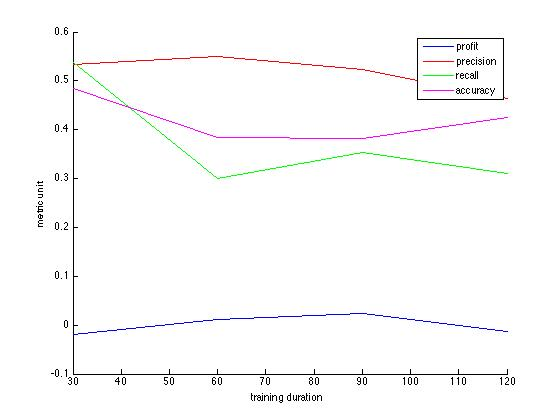
\includegraphics[width=0.45\textwidth]{tfreg_train}
\end{figure}

Hence, we train the logistic regression model with feature (1) and feature (4), starting from 9:30 AM to 10:30 AM, and the obtained model obtains precision $55.07\%$, recall $30.05\%$, accuracy $38.39\%$, and profit $0.0123$ when testing for the rest of the day.

\subsubsection{Improvements based on Time Locality}
While logistic regression was able to achieve a reasonable performance with the two-dimensional feature set including (1) and (4) and made a profit of $0.0123$ , we attempted to further improve our results. Based on earlier discussion, our logistic regression model is constrained to a low-dimensional feature space. As a result, we must either select more descriptive features in low-dimensional feature space or use a different model that would learn from a higher-dimensional feature space for our application.\\ 

We started by constructing more descriptive features. We hypothesized that the stock-market exhibits significant time-locality of price-trends based on the fact that it is often influenced by group decision making and other time-bound events that occur in the marketplace. The signals of these events are usually visible over a time-frame longer than a minute since in the very-short term, these trends are masked by the inherent volatility of the stock prices in the market. For example, if the market enters a mode of general rise with high-fluctuation at a certain time, then large 1-minute percentage changes in price or volume become less significant in comparison to the general trend.\\

We attempted to address these concerns by formulating new features based on the $\lambda$-minute high-low model\footnote{Inspired by CS 246 (2011-2012 Winter) HW4, Problem 1.}. Professionals in the algorithmic trading field recommended the heuristic choice of $\lambda=5.$\footnote{Keith Siilats, a former CS 246 TA} The $\lambda$-minute high-low model tracks the high price, low price, high volume, low volume across all the ticks in any $\lambda$-minute span. For the most recent $\lambda$-minute span w.r.t. any 1-minute bucket of time $t$, we define $PH_{\lambda}^{(t)}$, $PL_{\lambda}^{(t)}$, $VH_{\lambda}^{(t)}$, $VL_{\lambda}^{(t)}$ as follows:
\begin{eqnarray}
PH_{\lambda}^{(t)} &=& \maxx{t - \lambda \leq i \leq t - 1}P^{(i)}_{high} \\
PL_{\lambda}^{(t)} &=& \minx{t - \lambda \leq i \leq t - 1}P^{(i)}_{low} \\
VH_{\lambda}^{(t)} &=& \maxx{t - \lambda \leq i \leq t - 1}P^{(i)}_{high} \\
VL_{\lambda}^{(t)} &=& \minx{t - \lambda \leq i \leq t - 1}P^{(i)}_{low}
\end{eqnarray}

Under the $\lambda$-minute high-low model, we choose our features to be the following:
\begin{eqnarray}
\frac{\left(P_{open}^{(t)} - P_{open}^{(t-1)}\right)}{PH_\lambda^{(t)}-PL_\lambda^{(t)}} \\
\frac{\left(V_{open}^{(t)} - V_{open}^{(t-1)}\right)}{VH_\lambda^{(t)}-VL_\lambda^{(t)}}
\end{eqnarray}

Specifically, they are the ratio of open price and open volume change to the most recent ``$\lambda$-minute high-low spread", respectively.\\

Considering that our stock universe may be different, we use cross-validation to determine the optimal value of $\lambda$. Figure 2 suggests that $\lambda=5$ leads to maximal precision while $\lambda=10$ guarantees maximal profit and recall. For the purpose of this project, we chose $\lambda=5$ because higher precision leads to a more conservative strategy.
\begin{figure}[H]
\caption{Performance over different $\lambda$}
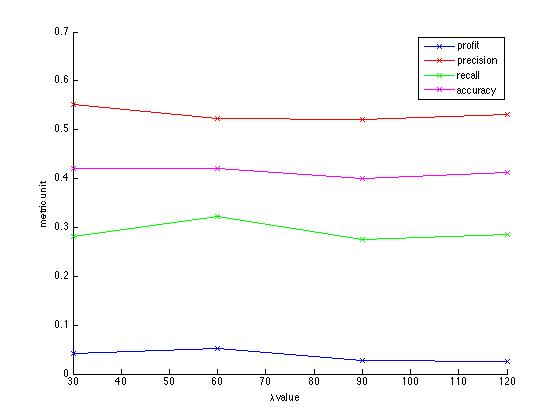
\includegraphics[width=0.45\textwidth]{lambda_reg}
\end{figure}
Also, we set training duration to 60 minutes based another cross-validation analysis with $\lambda=5$. Our $\lambda$-minute high-low logistic regression model finally achieves precision $59.39\%$, recall $27.43\%$, accuracy $41.58\%$ and profit $0.0186$.

\begin{table}[H]
\centering
\caption{Comparison between two logistic regression models}
\begin{tabular}{ c|c|c|c|c }
 Model  & Profit & Precision & Recall & Accuracy \\
\hline
\hline
Baseline & 0.0123   &     $55.07\%$  &    $30.05\%$   & $38.39\%$  \\
$\lambda$-HL    &    0.0186     &   $59.39\%$   & $27.43\%$   &  $41.58\%$ \\
\hline
\end{tabular}
\end{table}

By compare the performance of the two logistic regression models in Table 1, we clearly see that $\lambda$-minute high-low model provides a superior model than baseline model. This result validates our hypothesis on the time-locality characteristic of stock data and suggests that time-locality lasts around 5 minutes.

\subsection{Support Vector Machine}
As we discussed earlier, further improvement of results may still be possible by exploring a new machine learning model. The previous model we explored contained us to a low-dimensional feature space, and to overcome this constraint, we attempted to experiment with \textbf{SVM using $\ell$-1 regularization with $C = 1$}.

\subsubsection{Feature \& Parameter Selection}
We tried different combinations of the 8 features defined by equation (1) to (6), equation (11), and equation(12). Since there are a large number of feature combinations to consider, we used forward-search to continuously add features to our existing feature set and choose the best set based on our 4 metrics.
\begin{table}[H]
\centering
\caption{Performance over different feature sets}
\begin{tabular}{ p{2cm}|c|c|c|c }
 Features  & Profit & Precision & Recall & Accuracy \\
\hline
\hline
(1), (4) & 0.3066   &     $44.72\%$  &    $52.11\%$   & $42.85\%$  \\
\hline
(11), (12) &    0.3706     &   $42.81\%$   & $57.64\%$   &  $40.34\%$ \\
\hline
(1), (4), (11), (12) &    0.3029     &   $42.48\%$   & $47.54\%$   &  $39.42\%$ \\
\hline
(1), (4), (11), (12), (2), (5) &    0.3627     &   $45.22\%$   & $56.25\%$   &  $42.60\%$ \\
\hline
(1), (4), (11), (12), (2), (5), (3), (6) &    0.3484     &   $46.43\%$   & $55.66\%$   &  $42.91\%$ \\
\hline
\end{tabular}
\end{table}
We chose the last feature set since it leads to the highest precision and also very high profit, recall, and accuracy. In addition, we set training duration to 60 minutes using cross-validation. Similarly, we choose optimal $\lambda=10$ and $C=0.1$ using cross-validation. We also compared linear kernel with Gaussian kernel, and linear kernel tends to give better results.\\

The SVM model trained with the chosen training duration, $\lambda$ and $C$ finally achieves precision $47.13\%$, recall $53.96\%$, accuracy $42.30\%$ and profit $0.3066$. By comparing $\lambda$-minute high-low regression model with SVM model, we see that SVM model significantly improves recall, by almost 100\%, by only sacrificing a small percentage of precision, around 20\%.

\subsubsection{Time-Locality Revisited}
Recall that the $\lambda$-min high-low model is based on our hypothesis that there exists a $\lambda$ minute rolling correlation in between trades within a certain period of time, and by cross-validation, we choose $\lambda=10$ for the SVM model. To further substantiate this hypothesis, we conducted an experiment in which we train an SVM using the optimal parameters from the previous section, and then we evaluate the accuracy of the model by testing it on different periods of time.\\

Specifically, the performance statistics of an SVM model, trained from 9:30 AM to 10:30 AM, are listed in Table 3. A close inspection shows that there exists a downtrend in performance as delay between testing period and training period becomes larger. In fact, it wouldn't be surprising to see even better performance of this model within 10 minutes after training completes as we chose $\lambda=10$\footnote{The result is precision: $68.84\%$, recall: $36.88\%$, accuracy: $44.84\%$, which tops all other results in Table 3.}!

\begin{table}[H]
\centering
\caption{Performance over periods of time}
\begin{tabular}{ p{2cm}|c|c|c|c }
 Period  & Profit & Precision & Recall & Accuracy \\
\hline
\hline
10:30-11:00 AM &    0.0926     &   $56.45\%$   & $38.10\%$   & $43.92\%$  \\
\hline
10:45-11:15 AM &    0.0684     &   $42.49\%$   & $38.32\%$   &  $42.15\%$ \\
\hline
11:00-11:30 AM &    0.0775     &   $54.29\%$   & $41.09\%$   &  $43.07\%$ \\
\hline
11:15-11:45 AM &    0.0726     &   $48.68\%$   & $36.68\%$   &  $38.68\%$ \\
\hline
11:30-12:00 AM &    0.0632     &   $32.74\%$   & $29.77\%$   &  $40.44\%$ \\
\hline
\end{tabular}
\end{table}

\section{Conclusion}
We have applied successfully a segmentation and tracking model for hand-held
camera data to RGBD data captured by autonomous car.
By trial and error we have gained a deep understanding of the model, 
the effects of different features, and SSVM setup. Due to time limit of a class
project, we did not have time to experiment with more features that are more
specific to the nature of autonomous car data. For example,
we cannot calculate surface normal for a lot of far away depth points, because
they do not have neighbors with which we can estimate the plane. If we had
time, we could 
develop a new feature that computes the tangent through a few nearby points
in the same depth ring to replace surface normals. Also, adding surface normal alone still does not get rid of all the points on the ground that touch the tracked objects. We may solve this problem by first applying ground subtraction, and then run our segmentation pipeline.
 However, the current result is satisfying both qualitatively and quantitatively.
 We believe the application of an improved version of the algorithm can help
 autonomous cars be more knowledgeable about the different kinds of obstacles 
 and make finer-grained decisions in all kinds of traffic situations.

%-------------------------------------------------------------------------

{\small
\bibliographystyle{ieee}

\begin{thebibliography}{20}
\bibitem{AlexRGB}
  Alex Teichman, Sebastian Thrun,
  Learning to Segment and Track in RGBD.

\bibitem{AlexDepth}
  Alex Teichman, Sebastian Thrun,
  Tracking-Based Semi-Supervised Learning.

\bibitem{SSVM9}
T. Joachims, T. Finley, and C.-N. Yu. Cutting-plane training of structural svms. Machine
Learning, 77(1):2759, 2009.

\bibitem{SSVM20}
M. Szummer, P. Kohli, and D. Hoiem. Learning crfs using graph cuts. In ECCV, 2008.

\bibitem{SSVM21}
21. B. Taskar, V. Chatalbashev, D. Koller, and C. Guestrin. Learning structured prediction models:
A large margin approach. In ICML, 2005.

\end{thebibliography}

\bibliography{egbib}
}

\end{document}
